%----------------------------------------------------------------------------------------
\begin{frame}
  \frametitle{DHIT{\small Decay of Homogeneous Isotropic Turbulence}}
  \textbf{Problem setting:}
  \begin{itemize}
  \itemsep0cm
  \item Prescribed initial energy spectra corresponding to $Re_{\lambda}=952$
  \item Setting defined in AGARD database [Mansour \& Wray, 1993]
  \item Different mesh discretizations ($ Q_1/Q_1 $ and $ Q_2/Q_2 $)
  \end{itemize}
  \vspace{-0.1cm}
  \begin{figure}
      \centering	
      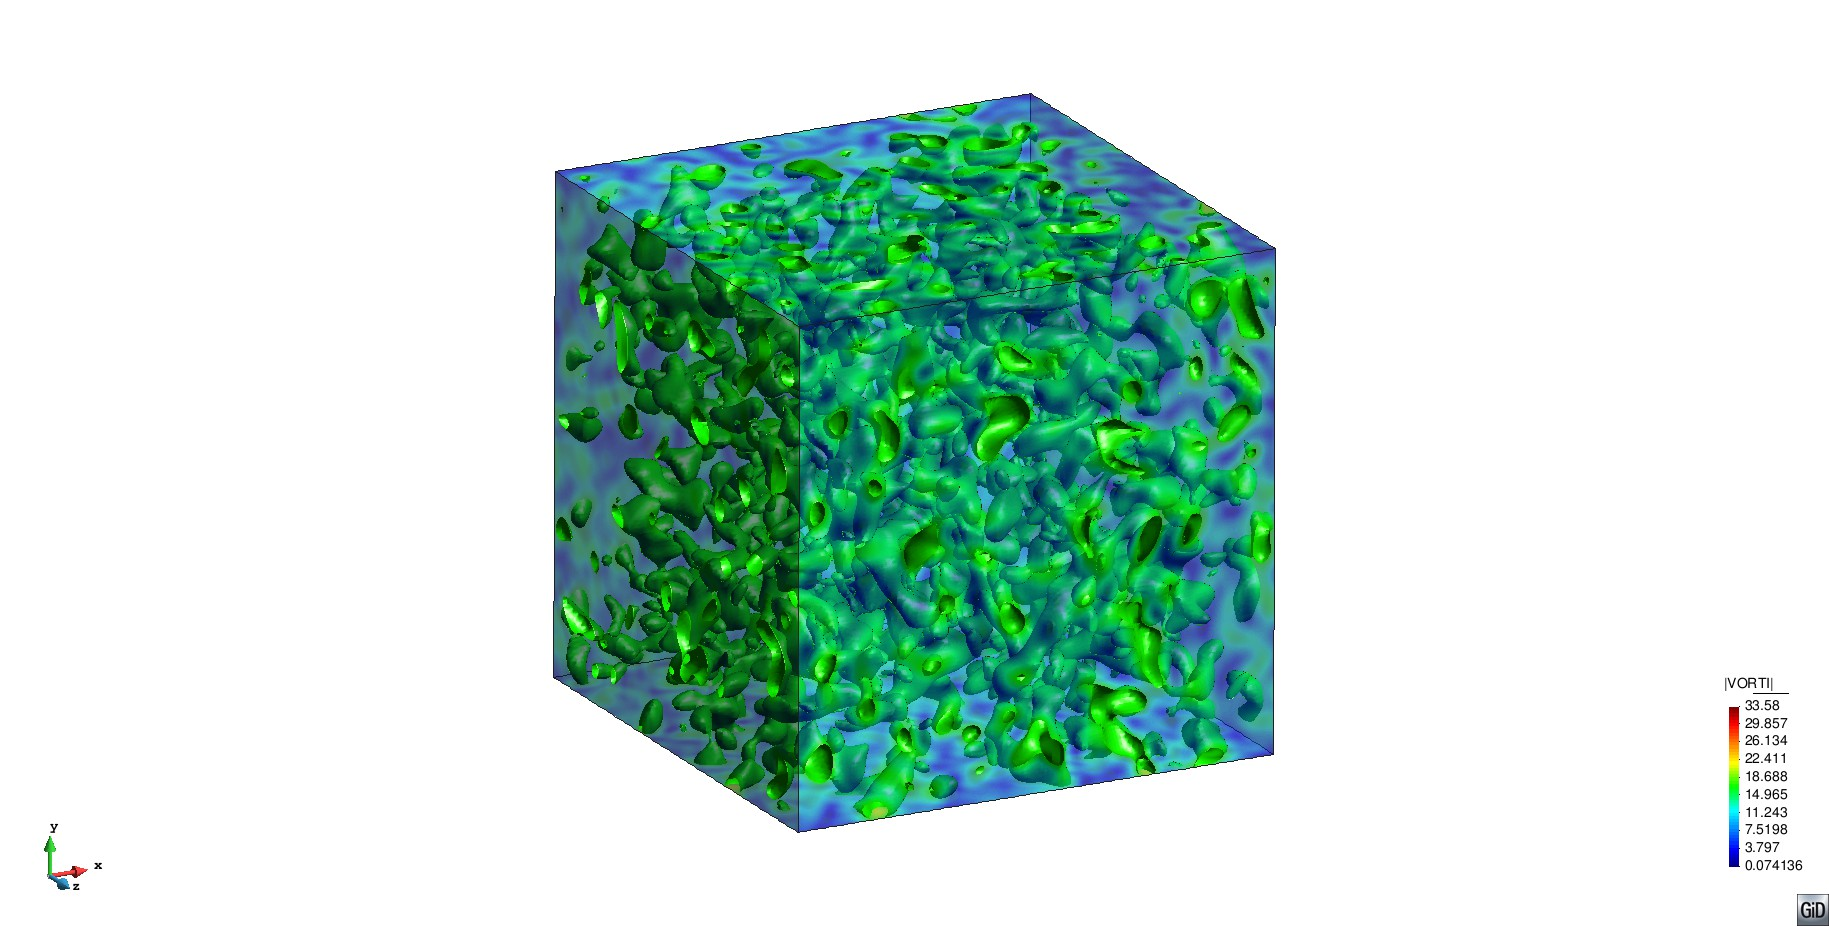
\includegraphics[clip=true,trim=19cm 2cm 19cm 3cm,width=0.45\textwidth]{Figures/iso_vorti_1.jpg}
  \end{figure}
\end{frame}
%----------------------------------------------------------------------------------------
\begin{frame}[t]
  \frametitle{DHIT{\small Decay of Homogeneous Isotropic Turbulence}}
  \textbf{Energy espectra (models):}
  \vspace*{-1.0cm}
  \begin{columns}
  \begin{column}{0.5\textwidth}
  \begin{figure}
    \centering	
    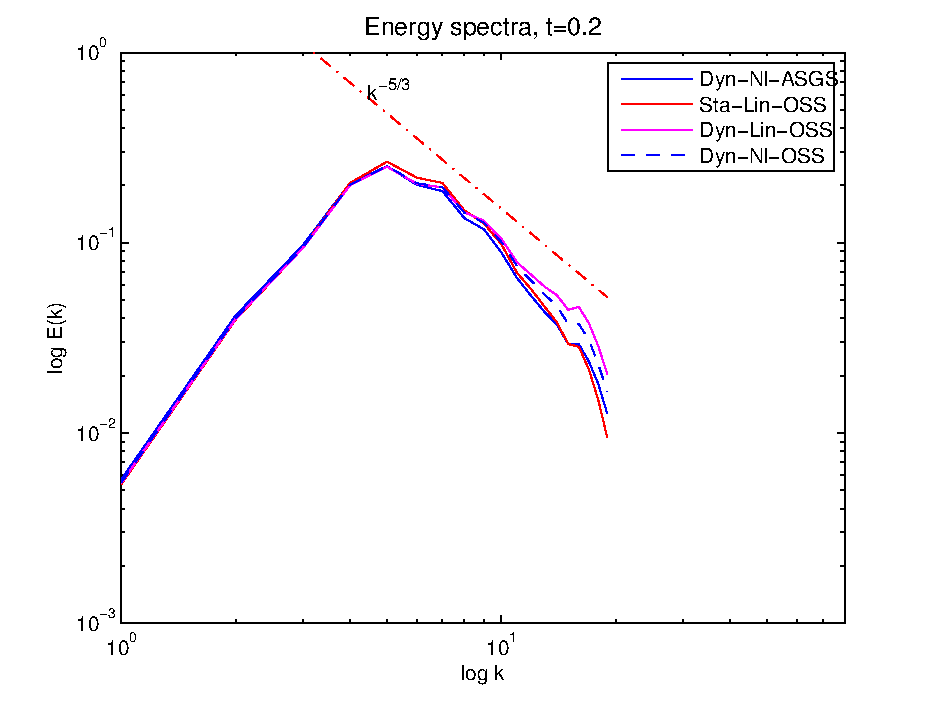
\includegraphics[width=1.1\textwidth]{Figures/spec_32_02_scaled}
    \vspace*{-0.8cm}
    \caption{$32^3-Q1$, $t=0.2s$}
  \end{figure}
  \end{column}
  \begin{column}{0.5\textwidth}
    \begin{figure}
    \centering	
    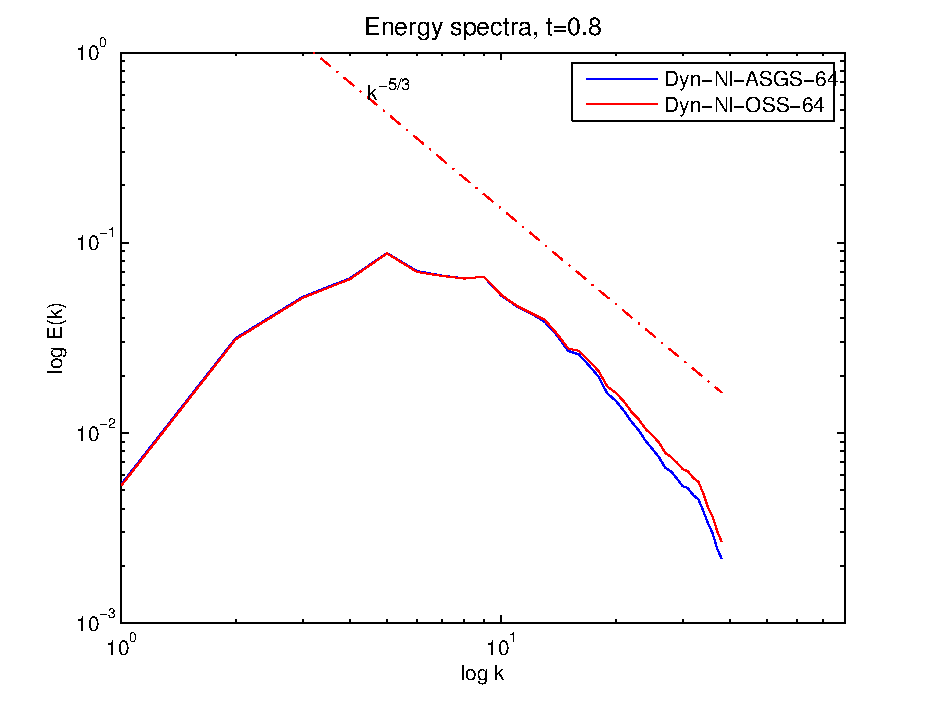
\includegraphics[width=1.1\textwidth]{Figures/spec_64_08}
    \vspace*{-0.8cm}
    \caption{$64^3-Q1$, $t=0.8s$}
  \end{figure}
  \end{column}
  \end{columns}
  \vspace*{-0.3cm}
  \begin{overlayarea}{\textwidth}{1.5cm}
  \only<2->{
  \begin{itemize}
  	\item \alert<2>{Small differences} between methods (physical sense)
  	\only<3->{\item Even \alert<3>{more similar when we refine} the mesh}
  \end{itemize}}
  \end{overlayarea}
\end{frame}
%----------------------------------------------------------------------------------------
\begin{frame}
\frametitle{DHIT{\small Decay of Homogeneous Isotropic Turbulence}}
\textbf{Computational cost (models):}
 \vspace*{-1.0cm}
 \begin{columns}
 \begin{column}{0.5\textwidth}
 \begin{figure}
  \centering
  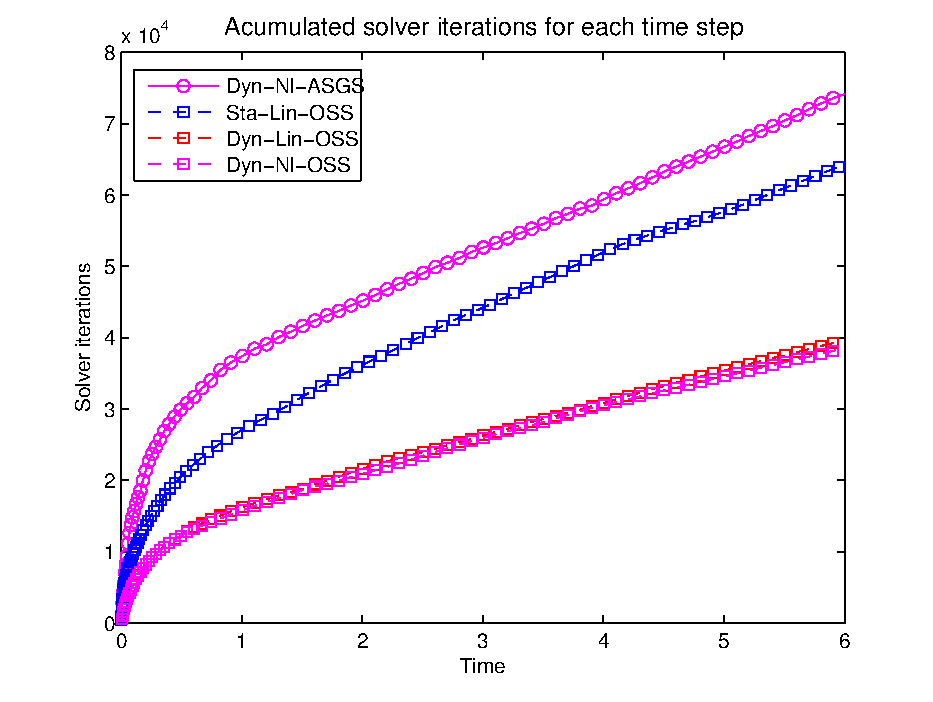
\includegraphics[width=1.1\textwidth]{Figures/Acsoliter_32_scaled_cnvgd}
      \vspace*{-0.8cm}
  \caption{$32^3-Q1$}
  \end{figure}
  \end{column}
  \begin{column}{0.5\textwidth}
   \begin{figure}
  \centering
  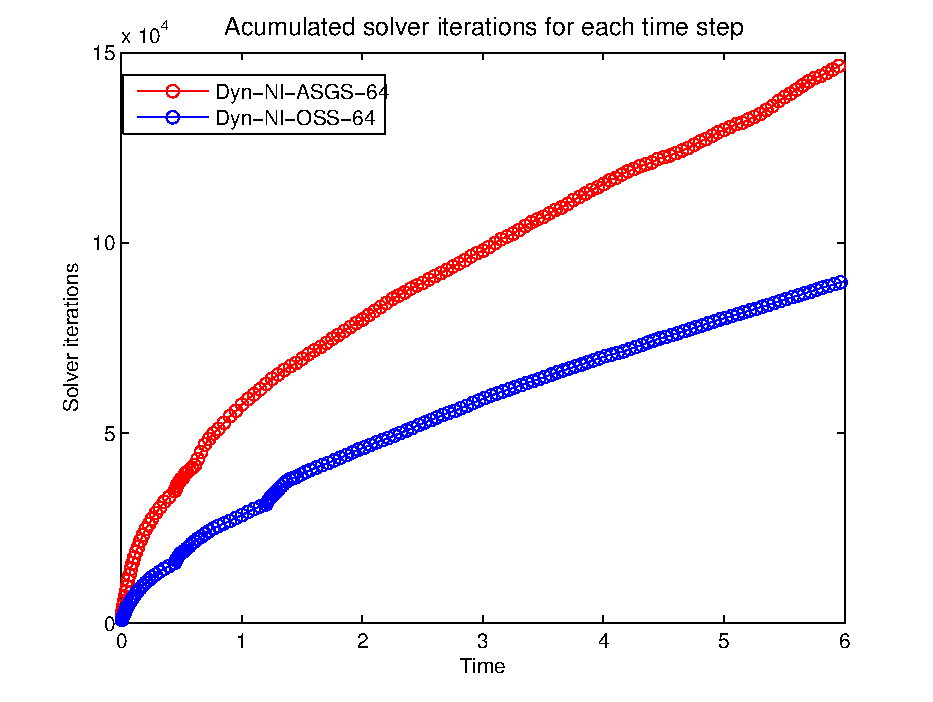
\includegraphics[width=1.1\textwidth]{Figures/Acsoliter_64}
      \vspace*{-0.8cm}
  \caption{$64^3-Q1$}
  \end{figure}
  \end{column}
  \end{columns}
  \begin{overlayarea}{\textwidth}{1.5cm}
  \vspace*{-0.3cm}
  \only<2->{
  \begin{itemize}
  	\item \alert<2>{Big differences} between methods (computational sense)
  	\only<3->{\item \alert<3>{Dynamic} versions of \alert<3>{OSS} method are \alert<3>{the most efficient}}
  \end{itemize}}
  \end{overlayarea}
\end{frame}
%----------------------------------------------------------------------------------------
\begin{frame}[t]
  \frametitle{DHIT{\small Decay of Homogeneous Isotropic Turbulence}}
  \textbf{Energy espectra (refinement):}
  \begin{figure}
    \centering	
    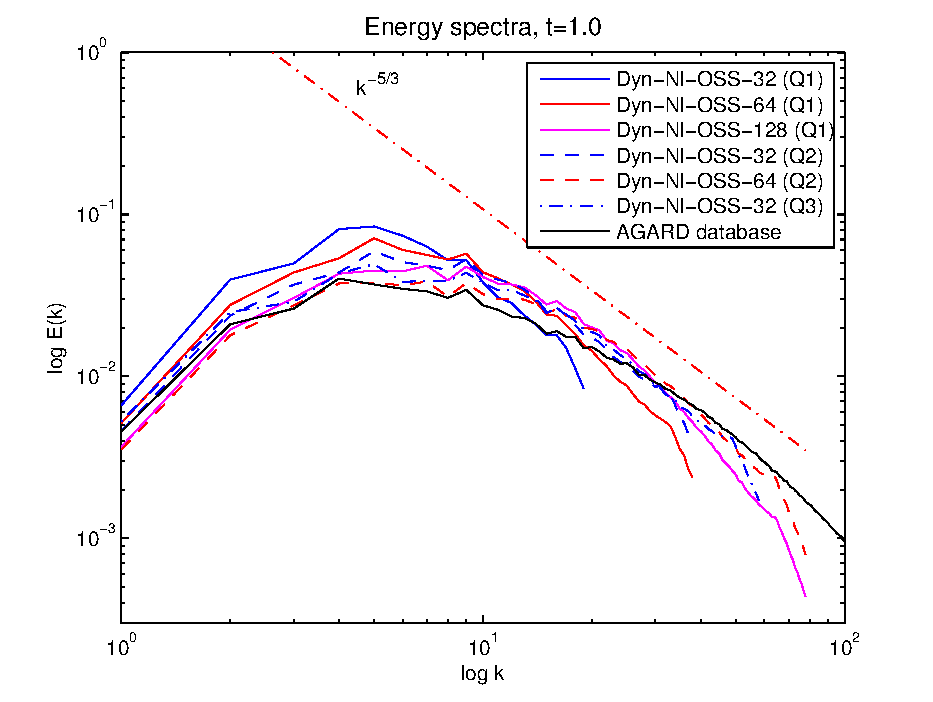
\includegraphics[width=0.7\textwidth]{Figures/spec_hp_1}
  \end{figure}
  \begin{overlayarea}{\textwidth}{1.5cm}
  \vspace*{-0.6cm}
  \begin{itemize}
  	\item Results become \alert<1->{closer to the DNS when we refine} the mesh
  \end{itemize}
  \end{overlayarea}
\end{frame}